% Imporditud: tools/import_eksperimendid.py
% Allikas: Eesti füüsikaolümpiaadi eksperimendi ülesannete
%   kogu (Rael Kalda, 2023), ülesanne Ü146, lahendus L146.
\setAuthor{Eero Uustalu}
\setRound{lõppvoor}
\setYear{2014}
\setNumber{G E1}
\setDifficulty{4}
\setTopic{geomeetriline optika}
\setVahendid{Fresneli lääts, mõõdulint, vesi (murdumisnäitaja nvesi = 1,33), läbipaistev plaat, kuivatuspaber}
\setPunktid{12}
\setAllikas{Eksperimendi kogu Ü146, lahendus lk 108}
\setLahendusseis{toores}

\prob{Fresneli lääts}
Määrake Fresneli läätse materjali absoluutne murdumisnäitaja nf .
\begin{center}
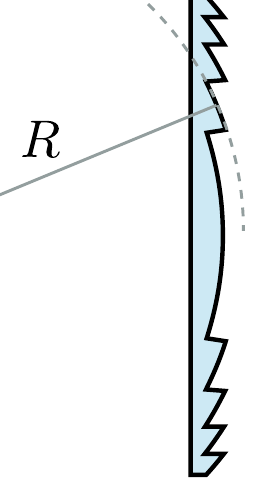
\includegraphics[width=0.22\linewidth]{2014-v3g-ge1-yl.png}
\end{center}
\textit{Näpunäited:} Selles katses kasutatava Fresneli läätse üks pind on tasane ning teine koosneb kaarjatest segmementidest raadiusega R (joonis läbilõikest). Fresneli läätse sakilise pinna võib asendada mõttelise sfäärilise pinnaga, mille kõverusraadius on samuti R, ilma et läätse fookuskaugus sellest muutuks. Tasakumera läätse optiline tugevus avaldub kui D = (n$-$1)/R, kus n on läätse materjali murdumisnäitaja ümbritseva keskkonna suhtes. Üksteisega kokkupuutuvatest optilistest elemetidest koosneva süsteemi optiline tugevus avaldub süsteemi elementide optiliste tugevuste summana.

\hint

\solu
Määrame läätse fookuskauguse.

1 (n $-$ 1) fL = DL = R

Täidame läätse hammastatud poole ja läbipaistva plaadi vahe veega, mille tulemusena saame litläätse. Nüüd määrame selle liitläätse fookuskauguse. Lahutame selle kaheks lähedal asetsevaks iseseisvaks läätseks, kus negatiivse vesiläätse optiline tugevus on

1 = Dv = (nv $-$ 1) fv $-$R

Selle läätsesüsteemi optiline tugevus ja fookuskaugus on

1 = Ds = DL + Dv = (n $-$ 1) + (nv $-$ 1) = (n $-$ nv) fs R $-$R R

Seega

1 = (n $-$ 1) ja 1 = (n $-$ nv) fL R fs R

Lahendame süsteemi ja avaldame murdumisnäitaja n = nv $\cdot$ fs $-$ fL fs $-$ fL

Kui fs = 0,43 m ja fL = 0,15 m, siis n = 1,507.

Märkus: Kaugete objektide puudumisel peaks fookuskauguse täpseks määramiseks

kasutama läätse valemit 1 11 =+

f ak

kus f on fookuskaugus, a esemekaugus läätsest ning k kujutise kaugus läätsest.
\probend
